% REMEMBER: You must not plagiarise anything in your report. Be extremely careful.
\documentclass{l4proj}
\usepackage{adjustbox}
    
%==============================================================================
% Put any additional packages here
% You can add any packages you want, as long as it does not alter
% the overall format (e.g. don't change the margins or the reference style).
%
\usepackage{pdfpages} % if you want to include a PDF for an ethics checklist, for example
%
%

\begin{document}

%==============================================================================
%% METADATA
\title{Controlling Two Characters Using Reinforcement Learning with Physics} % change this to your title
\author{Julian Lee}
\date{July 31, 2024}

\maketitle

%==============================================================================
%% ABSTRACT
\begin{abstract}
    DeepMimic is a deep reinforcement learning physics-based character animator that is hasn't implemented multiple character interactions. This project aims to discover if it is possible to implement multiple character interactions and apply reinforcement learning to make simulation more stable. The purpose of this was to further advance the projects that apply deep reinforcement learning such that they can be more widely used.
\end{abstract}

%=============================================================================
%% ACKNOWLEDGEMENTS
\chapter*{Acknowledgements}
% Enter any acknowledgements here. This is optional; you may leave this blank if you wish,
% or remove the entire chapter
%
% We give thanks to the Gods of LaTeX, who in their eternal graciousness, 
% have granted that this document may compile without errors or overfull hboxes.
%
Thank you to my supervisor for his eternal patience and kindness.
%==============================================================================

% EDUCATION REUSE CONSENT FORM
% If you consent to your project being shown to future students for educational purposes
% then insert your name and the date below to  sign the education use form that appears in the front of the document. 
% You must explicitly give consent if you wish to do so.
% If you sign, your project may be included in the Hall of Fame if it scores particularly highly.
%
% Please note that you are under no obligation to sign 
% this declaration, but doing so would help future students.
%
%\def\consentname {My Name} % your full name
%\def\consentdate {20 March 2018} % the date you agree
%
\educationalconsent


%==============================================================================
\tableofcontents

%==============================================================================
%% Notes on formatting
%==============================================================================
% The first page, abstract and table of contents are numbered using Roman numerals and are not
% included in the page count. 
%
% From now on pages are numbered
% using Arabic numerals. Therefore, immediately after the first call to \chapter we need the call
% \pagenumbering{arabic} and this should be called once only in the document. 
%
%
% The first Chapter should then be on page 1. 

% PAGE LIMITS
% You are allowed 40 pages for a 40 credit project and 30 pages for a 
% 20 credit report. 
% This includes everything numbered in Arabic numerals (excluding front matter) up
% to but *excluding the appendices and bibliography*.
%
% FORMATTING
% You must not alter text size (it is currently 10pt) or alter margins or spacing.
% Do not alter the bibliography style. 
%
%==================================================================================================================================
%
% IMPORTANT
% The chapter headings and structure here are **suggestions**. You don't have to follow this model if
% it doesn't fit your project. Every project should have an introduction and conclusion,
% however.  If in doubt, your supervisor can give you specific guidance; their view takes precedence over
% the structure suggested here.
%
%==================================================================================================================================
\chapter{Introduction}

% reset page numbering. Don't remove this!
\pagenumbering{arabic} 

\section{Character Animation}
This is a dissertation about the ability to control multiple character interactions with physics using reinforcement learning. Character animation is a key component of digital entertainment, which has a major influence on the movie, game, and VR/AR industries. It entails designing believable actions for virtual characters to make the overall experience more engaging to the viewers.

\section{A History of Character Animation Techniques}
Techniques used in character animation have changed significantly over the years from the use of hand drawings to more advanced CGI. We see examples of this in companies like the Walt Disney Animation Studios, which started out producing hand drawn animations like The Fox and the Hound (1981) and Mulan (1998). This all changed when the first fully computer animated feature was put out, Toy Story(1995), being met with rave reception and making a massive amount of money, becoming one of the top 100 grossing movies. Since then, CGI films have been put out more and more, such as as Frozen (2013), becoming the norm nowadays.

This isn't to say that character animation is important only in animated films. Films which are live-action need CGI as well. A good example of this is the Star Wars franchise, which had been using puppets for aliens such as Yoda in the original trilogy. However, this changed in the prequel trilogy, where the director George Lucas made the choice to make Yoda into a fully CGI character, so that the character could move about and flip around in battle.

Nowadays, many mediums use Motion Capture, or mocap, to help to automate the process of animating characters. This involves putting a tracking suit on an actor or stand in, and tracking their movements while they act. This can be used to stunning effect, such as the depiction of Davy Jones in Pirates of the Caribbean 2 (2006). The usage of mocap allowed them to make an amazing visual effect that still holds up today, all while keeping Davy Jones expressive and dynamic. Mocap doesn't just make the process of making characters easier, it also allows creators to be more accurate.
\clearpage
\section{Importance in Digital Entertainment}
In the film industry, character animation is used to make animated characters more realistic and thus more appealing to the viewers. This technique has been essential in creating large-scale movies with complicated characters that include computer-generated imagery. One only needs to look at the Marvel Cinematic Universe to see the expansive amount of CGI used, with studios investing millions of dollars for VFX studios to enhance their film as described by \cite{tina23}.

In gaming, realistic character animations are crucial for improving the level of interaction between the player and the game, making it more enjoyable. The race to develop the best looking game to attract an ever-growing player base has been rapidly ongoing. Graphics play a big part in the enjoyment of a video game, but just texture alone is not enough to make a game stand out. A game that has good physics, how a character can interact with a world, is often met with praise. One look at a recent game that came out, Guily Gear -Strive- (2021). The need for good character animation in fighting games, where two characters interact with each other by blocking, and hitting each other, is very important. This is due to the main focus of these games being very character and frame focused. \cite{guiltygear23} says that movements must be responsive, and animations tight, to keep users feeling like the game is good to play and not frustrating. However, good character animation often makes development harder. A good example of this is a recent game, Stellar Blade (2024). The game is again very focused on character animation, particularly the main draw of the game, that being Eve, the main player character. A single-player "beat-'em-up" game, where players control a character to fight numerous non-playable characters. As a result, focus is placed on the main character, whether or not they look good, whether the physics hold up, and whether they feel good to play. The director of Stellar Blade, Hyun-Tae Kim, admitted that the character design hampered development, due to the main character's long ponytail, which was difficult to get to bounce and sway naturally. Kim goes on to jokingly say that development time could have been cut down by a year, reported \cite{dexerto24}.

The use of realistic character animation is crucial in VR/AR applications to enhance the presence and overall experience in virtual reality. An example of this going very wrong would be a first look at Mark Zuckerberg's product, Metaverse. Much like good character animation can enhance a user experience, bad character animation can greatly diminish it. The Metaverse was supposed to be an ambitious project that attracted millions of users, and its creators, Facebook, invested heavily in it. This would turn out to be a mistake, which became apparent as soon as they had their first presentation. It was met with ridicule online, with talks about how bad the characters looked, comparing it to pre-existing VR software such as VRChat. \cite{wagner23} goes on to explain that the project, which had billions invested in it wasted, became the laughing stock of the internet and the project has floundered ever since. 

From these examples, we see that an important key to engaging with your audience is good character animation. Projects might be judged based on how a customer first perceives it, and if a customer sees strange physical movements, they might be less inclined to try out a product. Moreover, customer retention might be based on character animations. Drawing from the previous fighting game example, if your game does not have good animation, a user could get frustrated or disinterested in your game and go to one of the many other products in the field. However, there is a cost to implementing good character animation, whether it be from the time spent working on it, to the money sunk into developing your project, such as hiring VFX studios for movies and the hardware required to run your program.

%==================================================================================================================================
\chapter{Background}

\section{Techniques}
When we talk about character animation, we tend to be talking about specific methods that have been popularised over the recent century.

\subsection{Keyframe-Based}
One of the earliest methods ever developed was keyframe-based animation. This is where the animator designs keyframes for important positions within the animation and the computer generates the frames in between resulting in a smooth motion, described by long-time professional animator \cite{survival09}. Keyframe animation is time-consuming, and only looks natural when a lot of effort and talent is being put into it. However, it requires less calculations than other methods, making it a versatile medium for artists to use.

A good example of this would be our previous example of Guilty Gear Strive, the fighting game. Character animation there is more stylistic than other games, with a specific cartoon art style in a pseudo 2D-world. As a result, the animators use keyframes to get a character in a position that looks good from the direction of the camera, even if logically, the position doesn't make any sense, stretching limbs and resizing them. This is a common animation trick to make movements seem more expressive, as told in the twelve basic principles of animation by \cite{disneyanimation81}.

\subsection{Kinematic-Based}
Kinematic animation can either employ forward kinematics, or inverse kinematics.

\cite{Paul1981-ar} states that forward kinematics are used primarily in robot kinematics. The goal of the kinematic equations being used calculates the position of the end of a limb from specified values for the joint parameters. These equations can also be used in other sectres, like computer games, and animation. In terms of character animation, the motion of the model is defined by the animator, ignoring variables such as gravity or unexpected collisions.

Inverse kinematics uses specified end points to control the position and orientation of a character's limbs, being like the opposite of the afformentioned forward kinematics. Characters are more easily able to react to changes in environment around them, such as uneven ground, which was revealed in a paper by \cite{Lee1999}. They describe in their paper how traditional inverse kinematics was very computationally expensive, but allowed them a level of adaptibility that was novel at the time. While inverse kinematics is adaptable, it's also less accurate for precise movements in character animation. The reason for this lies in the calculation of the joints based on the end point. Technically speaking, as long as the joint reaches the end point, the solution is correct. This can lead to multiple solutions, lowering accuracy.

\subsection{Relationship Descriptor-based}
\cite{AlAsqhar2013} describes the process of using Relationship Descriptors, motion of a character can be retargeted to characters of different sizes or interact with objects of different shapes and sizes. \cite{AlAsqhar2013} goes on to compare their framework to previous kinematic-based discrete representations that only handle static spatial relationship or require costly optimisation processes, and shows that this works as a more cost-effective, automated method. They do this through the weighted sum of translation vectors relative to points selectively sampled over the surfaces of mesh structures.

\subsection{Physics-Based Simulation}
Physics based animation techniques involve the use of physical principles that control the motion of real objects to produce more realistic character movements. In contrast to kinematic and keyframe-based approaches which involve keyframes and animator inputs, or the calculation of joints from endpoints, physics-based animation involves algorithms that incorporate forces like gravity, friction, and momentum, revealed by \cite{boeing07} in their paper. It also allows characters to perform actions and navigate through the space in a more realistic way. The realism and natural motion that are achieved through this technique is important in providing audiences with a believable experience, states \cite{Holden2017}. When animating a fully animated world, the familiar sense of something universal like gravity helps to ground the viewer and give them a more immersive experience.
\clearpage
\section{Reinforcement Learning in Character Animation}
In physics-based character simulation, we are able to use reinforcement learning (RL) to train a character to perform new tasks. Reinforcement learning is a process in which we can enhance the performance of a character based on trial and error. \cite{deepmimic}, one of the pioneers of this field, describes how he trains policies to help automate accurate animation. Take for example, a simulated character. The body of a character is called a ragdoll. Without the help of a pre-trained policy, the ragdoll will just end up falling to the ground. However, using motion data that we have, Peng states how we can iteratively guide a character into following through its proper motion, collecting samples, and giving minute adjustments that creates a policy for the character to use. Through this, the character adapts their actions based on the feedback received from a policy. One such program that implements this, which we will be focusing on, is DeepMimic, made by \cite{deepmimic}.

\section{DeepMimic: Example-Guided Deep Reinforcement Learning}
The DeepMimic paper by \cite{deepmimic} brings several major advancements to the field of character animation. It was one of the earlier works in its field. It proves that deep reinforcement learning could be applied to characters in order for them to learn various complex movements, that don't require help from animators like other methods do. Moreover, it allows us to utilise mocap data to train these characters, removing the need for an animator to spend time to tediously go through numerous animations. This process lead to animations that were not only visually realistic, but also dynamically stable. It allows us to use characters on rough terrain, and the character will adapt accordingly. It does this by running a training program on a set of motion data to generate a policy, using training sets and test sets. Samples are collected from these to see whether the character succeeds. Throughout the training, noise also introduced to make the movement more adaptable to various situations. Eventually, the policy retains enough samples that the character is able to achieve their goal even in harsh environments, such as obstructions or objects being thrown at it.

DeepMimic does come with its set of drawbacks, though. One such drawback is that policies for characters trained on motion files take a very long time. Peng states that a simple movement will take about 60000000 samples to train properly, which takes a day, and complex movements take even more than that. Using mpiexec, a total of 16 workers can be assigned, but it is assumed that any more than that and the program will be overwhelmed. If the training of a policy such as with a movement such as punching takes a day, two characters interacting with each other with similar movement would take much more. Peng also states that resuming training a policy is not exactly supported.

I chose to use DeepMimic on the advice of my supervisor, as well as the wide pre-existing userbase due to it being one of the oldest projects of its kind. with a wide userbase comes a wide range of documentation, fixes to any issues I might face in my implementation of what I want to do, or similar solutions to what I am thinking of. Additionally, DeepMimic is open-source, which means that it is much easier to use and expand upon compared to other propriatary software.
\clearpage
\section{Similar Projects}
\subsection{Supertrack: Motion Tracking for Physically Simulated Characters}
SuperTrack is a tool created by Ubisoft that aims to improve the realism of physically simulated characters with the help of improved motion tracking. \cite{Fussell2021} in their paper explain how they have applied supervised learning to enhance the motion tracking to make characters mimic human movements with precision. SuperTrack enhances the integration of motion capture data and physical simulations to provide smoother transitions and realistic animations. This technique greatly decreases the amount of artifacts and unrealistic motion that is characteristic of purely physics-based models, enhancing the reality and interactivity of virtual characters. \cite{Fussell2021} goes on to explain that unlike reinforcement learning methods, which have a theoretically infinite look-ahead horizon controlled by the discount factor, the look-ahead of their method is limited to their policy window size. Supertrack is also not open-sourced, so I am unable to use it.

\subsection{CALM: Conditional Adversarial Latent Models for Directable Virtual Characters}
CALM is another tool, created by NVIDIA. \cite{tessler2023calm} in their paper talks about how they also built on DeepMimic to create a method for learning a representation of movement that captures the complexity and diversity of human motion, while also providing a directable interface for controlling a character's movements. They specify that they focus this tool towards gaming, where rugged environments are common, and the need to adapt a character to an environment based on player expression of freedom is very important. However, this technique is new and struggles with precision training, where intricate movements are hard to learn.

\subsection{Carpet Rolling for Character Control On Uneven Terrain}
Carpet Rolling was used as a tool to automate character animation on harsh terrain. This is a non-physics-based method, instead relying on Relationship Descriptors. They solve the problem of terrain locomotion by adapting movement of a character to arbritrary shapes. \cite{Miller2015} goes on to state that this result is highly parallelizable, and easily runs on GPUS, automating trajectories and actions of hundreds of characters during runtime. However, this also has limitations, where characters may suffer from sharp turns or very steep terrain, resulting in bad movement.
\clearpage
\section{Issues}
With these tools, there tends to be a drawback in scalability. One of the massive drawbacks of DeepMimic currently is that the research is based on a single controller. A single controller means that only one character is able to be trained. This model performs well in the creation of realistic individual motion but are not efficient in creating interactions between many characters. The inability to train multiple characters at once is a drawback especially in situations where dynamic interactions are important, such as in gaming or virtual reality. Take an example of animations in a game where two characters are fighting. In a fighting game, as previously discussed, they might use forward kinematics to painstakingly map out movement of a character, to match the style they are going for.

\section{Goals}
Recent studies in the field of physics-based character animation show that there are substantial improvements in the generation of natural and realistic character motions. Some works, such as DeepMimic, have demonstrated that RL and DL can be used to create high-quality animations, as described in \cite{deepmimic}'s paper. However, the scalability of characters is an issue, reducing their usefulness especially in more complex interactive worlds where dynamic interactions are important such as in the gaming or virtual reality areas, as discussed by \cite{Holden2017}.

It is my goal to be able to scale DeepMimic to display, train and simulate multiple characters at once. Doing this might have big impacts on the character animation field, allowing animations to be more automated, while at the same time being realistic. In this way, we would be able to engage an audience more without having as much time or cost spent as with other methods. This project can also act as a basis for further advancements in the field of physics-based character animation.

%==================================================================================================================================
\chapter{Analysis of DeepMimic}
To implement a version of DeepMimic that accepts multiple characters, datasets containing mocaps of multiple people interactions have to be used. With this in mind, we must look into the format of DeepMimic's humanoid model, in case any different conventions are used. Additionally, we must look into why exactly DeepMimic is unable to implement multiple characters in their training. This might involve argument files. The parameters given to argument files might only accept one character, which is maybe where the bottleneck lies. However, it is more likely that the problem lies in the source code itself. To figure this out, we need to figure out how scenes are made, and characters are implemented. An interesting distinction to make would be if it is the display of motion files that is the issue, or the simulation of the characters, as perhaps displaying multiple characters is permitted, but the initialisation of simulated characters only allows for a single instance.

\section{Formatting of Joints}
When first looking at the github repository for DeepMimic\footnote{\url{https://github.com/xbpeng/DeepMimic}}, Peng states that the program uses its own humanoid model, a skeleton of joints that is in the format displayed in Figure \ref{fig:deepmimic_format}.

\begin{figure}[htb]
  \centering
  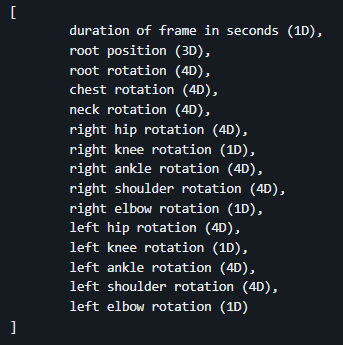
\includegraphics[width=0.5\linewidth]{images/deepmimic_humanoid_format.png}

  \caption{The format of a DeepMimic Humanoid, an array of the shape (No. of Frames, 44). Additionally, each of these elements correspond to a specific value, depending on their index. The 3 Dimension root position relates to X,Y,Z position of the root, while the 4 Dimension root orientation corresponds to quaternions for the global orientation of the root. The other 4 Dimension fields are quarternions, relating to the local rotation of their respective joints, and 1 Dimension fields are revolute joints corresponding to a scalar representation of the rotation of the joint in its respective axis as described by Peng.}

  \label{fig:deepmimic_format}
\end{figure}

However, this is a very unique format used to display rotation joints. One only needs to look at other formats to see that it is vastly different compared to others.

For instance, we can take the mocap dataset from CHI3D\footnote{\url{https://ci3d.imar.ro/}}, which uses a widely recognised skeleton format known as SMPL-X\footnote{\url{https://smpl-x.is.tue.mpg.de/}}. SMPL-X is a format derived from SMPL and SMPL-H, except with more populated joints for fingers and expressions as described by \cite{smplx19} in their paper. CHI3D is a dataset that uses mocap to track 2 humans interacting and represents them in these files.

When we extract the fields of the json file the mocap data comes in, we can see Figure \ref{fig:smplx_format}.

\begin{figure}[htb]
  \centering
  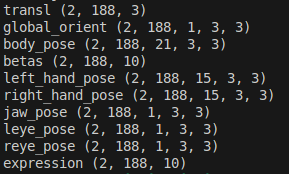
\includegraphics[width = 0.5\linewidth]{images/smplx_format.png}

  \caption{The format of an SMPL-X pictured in a mocap json file. We can see there's a transl field, relating to the root position, a global\_orient field which relates to global rotation of the root. Other than that, the joints we want to focus on are the local joint rotations pictured in the body\_pose field. In total, there are 21 joints in there. Joints are represented in a (3 $\times$ 3) rotation matrix. Additionally, the 2 fields at the start (2, 188) refer to the amount of characters and the amount of frames in a file.}

  \label{fig:smplx_format}
\end{figure}

DeepMimic has 13 joints, including the root. Meanwhile, the SMPL-X skeleton has 21 joints in total in body\_pose. We can see that there is a need to map the correct joints to their respective counterparts if we want to convert it to DeepMimic humanoid format. Not only that, but due to the lack of joints in the DeepMimic humanoid format, the SMPL-X movement is able to be much more expressive. As local joint rotations are related to their parent joint, losing some joints might translate very poorly as their parent joint is lost, replaced with the closest approximate we can find.

The differences in humanoids do not stop there, however. Due to a lack of convention in the community, axes are not necessarily correlative towards their counterparts. An example of this could be Figure \ref{fig:humanoids_in_program}.

\begin{figure}[htb]
  \centering
  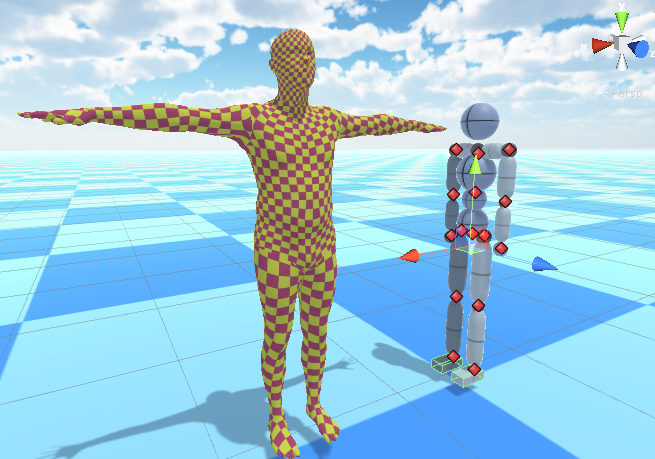
\includegraphics[width = 0.5\linewidth]{images/humanoids_in_program.png}
  
  \caption{Retrieved from DeepMimic Github, from user Zju-George. Pictured are the two humanoids on a plane of existence. The SMPL-X figure is on the left, T-Posing as its default position. The DeepMimic humanoid is pictured on the right, in its default position. On the top right is a compass, a legend for axes. This axes is related to this specific program.}
  
  \label{fig:humanoids_in_program}
\end{figure}

From Figure \ref{fig:humanoids_in_program}\footnote{url{https://github.com/xbpeng/DeepMimic/issues/72}}, we see that the default forward position of the SMPL-X figure is facing towards the Z-axis. The DeepMimic figure is facing towards the X-axis. This has implications towards the respective axes. For SMPL-X, the forward movement is Z-axis, while for DeepMimic, it is the X-axis. Axes convention difference means that changing one rotation such that it rotates around a certain axis would not necessarily translate towards the other respective joint.

Additionally, the default position for the rotation of the joints is different. We can see how the T-Pose, the default position of the SMPL-X figure differs from the arms down position of the humanoid. This affects local rotations of the joints. As an example of this, imagine the SMPL-X figure going from default T-Pose to its hands lowered down. The DeepMimic humanoid would also rotate about the same axis, but starting from its default, which means that their arms would actually rotate into the model.
\clearpage
\section{The Lack of Implementation of Multiple Characters}

\subsection{How DeepMimic Works}
The implementation uses C++ and Python, with a heavy majority leaning on C++. To run the code, argument files are passed on the type of character file, motion files, and what kind of scene is being run. Two scenes that I focused on are KinChar and Imitate scenes. KinChar scenes are a way to view how the motion file affects the joints of the characters, while Imitate scenes are what is used to simulate motion files and the policies that are related to them, which relate to the reinforcement learning of DeepMimic.

\subsection{Argument Files}
In the DeepMimic github repository, Peng describes how he has left examples of arguments in the folder \/arg, which are pictured in Figure \ref{fig:argfiles}. However, looking over the examples, one notices that there is not much documentation there, and thus if you wanted to add any extra fields or know how the arguments are parsed, you would have to go through the C++ and Python code. A clear example of this would be the argument to enable random character placement in the simulation sim. The argument file requires the parameter "enable\_rand\_char\_placement" with a boolean that returns false or true. However, in the example files that the github has, that variable is not present, as default initialisation of that variable is false and presumed not needed, thus not included in the argument files. If somebody wanted to enable random character placement, they would need to go through the scene initialisation, then to the argument parser for the screen drawn function. It is there that they will find argument parsing for enable\_rand\_char\_placement.

\begin{figure}[htb]
  \centering
  \begin{subfigure}[b]{0.45\textwidth}
    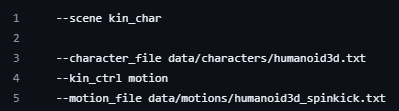
\includegraphics[width=\textwidth]{images/deepmimic_play_args.png}
    \caption{To play motion files}
    \label{fig:argfiles1}
  \end{subfigure}
  \begin{subfigure}[b]{0.45\textwidth}
    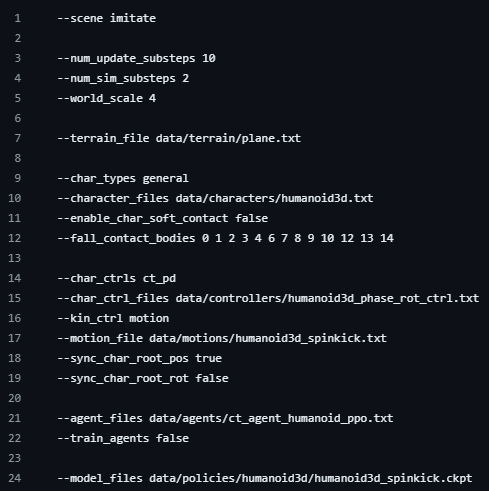
\includegraphics[width=\textwidth]{images/deepmimic_simulate_args.png}
    \caption{To simulate motion files and policies}
    \label{fig:argfiles2}
  \end{subfigure}
  \caption{Example Argument files given by Peng from the Github Repository for DeepMimic.}
  \label{fig:argfiles}
\end{figure}

A process of this begins in the initialisation of the scene that we want for training and simulation, scene type Imitate, seen in Listing \ref{lst:imitateinit}. From there, we realise that initalising SceneImitate calls RLSceneSimChar's initialisation in Listing \ref{lst:rlsiminit}, which in turn calls the initialisation function for SceneSimChar in Listing \ref{lst:siminit}.

\begin{lstlisting}[language=C++, float, caption={The Function that initialises Scene Imitate}, label=lst:imitateinit]
  void cSceneImitate::Init()
  {
		mKinChars[i].reset();
	  BuildKinCharacter();
	  BuildKinController();

	  cRLSceneSimChar::Init();
	  InitJointWeight();
  }
\end{lstlisting}

\begin{lstlisting}[language=C++, float, caption={The function that initialises RLSceneSimChar}, label=lst:rlsiminit]
  void cRLSceneSimChar::Init()
  {
    cRLScene::Init();
    cSceneSimChar::Init();

    mAgentReg.Clear();
    RegisterAgents();
    mAgentReg.PrintInfo();

    SetupTimerAnnealer(mTimerAnnealer);
  }
\end{lstlisting}

\begin{lstlisting}[language=C++, float, caption={The function that initialises SceneSimChar}, label=lst:siminit]
  void cSceneSimChar::Init()
  {
    cScene::Init();

    BuildWorld();
    BuildGround();
    BuildCharacters();

    InitCharacterPos();
    ResolveCharGroundIntersect();

    ClearObjs();
  }
\end{lstlisting}

It is finally in SceneSimChar that we find various argument parsing functions, including the argument we are searching for, which is just to enable random character placement, seen in Listing \ref{lst:simargparse}.

\begin{lstlisting}[language=C++, float, caption={The function that parses the arguments for SceneSimChar}, label=lst:simargparse]
  void cSceneSimChar::ParseArgs(const std::shared_ptr<cArgParser>& parser)
  {
    cScene::ParseArgs(parser);

    parser->ParseBool("enable_char_contact_fall", mEnableContactFall);
    parser->ParseBool("enable_rand_char_placement", mEnableRandCharPlacement);
    
    succ &= ParseCharTypes(parser, mCharTypes);
    succ &= ParseCharParams(parser, mCharParams);
    succ &= ParseCharCtrlParams(parser, mCtrlParams);

    ...
  }
\end{lstlisting}

This is just for an argument that affects the scene as a whole, which is why it is placed in the parse args overall function. However, if we wanted to see the fields for specific characters, for example, we would have to look at further functions that are called in Listing \ref{lst:simargparse}, like ParseCharParams() or ParseCharTypes().

Additionally, there is an inconsistency in the arguments in Figure \ref{fig:argfiles}. While the arguments for the KinChar scene call for "character\_file", the arguments for Imitate calls for "character\_files". This difference serves to confuse the user, and if you were to accidentally use the wrong one, the program throws a segmentation fault. Inconsistencies also occur in the error checking of arguments. For example, in the argument of "kin\_ctrl", the user just has to supplement one argument, that being the keyword "motion", and it would assign that type of kinematic control to multiple characters if it detected that there were more characters than kin\_ctrl specified. This is because there was an error check, where they checked the amount of arguments provided compared to character files. However, this does not hold true for "char\_ctrls", which requires a user to input a keyword like "ct\_pd". The more character files there are, the more the user has to enter an instance of ct\_pd. There is no error checking for this, and if the numbers don't match up, the program throws a segmentation fault.

\subsection{Initial Positions of Characters}
Then, we go into the initialisation of characters. Much like the argument issue above, initialisation of the characters can be altered to a few arguments. "enable\_rand\_char\_placement", would be assumed to make the program randomly place an initialised character around the world. With fixed placement, the character is initialised at the root of the world, which is represented in the XYZ format as (0,h,0). h corresponds to the height of the character root, such that the character won't be initialised halfway into the ground, or even under it. There is a way to offset the X-axis position of a character, by altering an argument field called "char\_init\_pos\_xs". Again, this is not in the example files given. 

Where we do find it is in the function that parses character parameters, which is logically where it should be parsed. This is shown in Listing \ref{lst:parsecharparams}.

\begin{lstlisting}[language=C++, float, caption={The function that parses the arguments for characters}, label=lst:parsecharparams]
  bool cSceneSimChar::ParseCharParams(const std::shared_ptr<cArgParser>& parser, cSimCharacter::tParams& out_params) const
  {
    ...
    std::vector<std::string> char_files;
    succ = parser->ParseStrings("character_files", char_files);

    std::vector<std::string> state_files;
    parser->ParseStrings("state_files", state_files);

    std::vector<double> init_pos_xs;
    parser->ParseDoubles("char_init_pos_xs", init_pos_xs);
    ...
  }
\end{lstlisting}

There is no other way to fine tune the initial position of the character spawned in. In all cases for fixed initial locations, the character is spawned at (0,h,0), unless the argument to change x is used. The argument to change x doesn't accept integers, however. It requires a double, which is in the format x.x, where x is a placeholder for any number. If a user put an integer x, or even a double in the format of (x.x) , the argument parser will skip over it. Due to the way it is implemented, it also doesn't throw any error messages, instead just ignoring the argument entirely. As a result, a user might be falsely led to believe that the offsetting of the x-axis just does not work.

\subsection{Display of Mocap Files}
For the display of motion files, without any physics, just relying on the joint rotations in the mocap dataset, argument files are presented as seen in Figure \ref{fig:argfiles1}. The initialisation function for DrawSceneKinChar is called, which launches the graphics user interface (GUI), displaying the character moving around. Initialisation for SceneKinChar is also called, which starts the motion file. Both the implementation of DrawSceneKinChar and SceneKinChar can only use one character. Listing \ref{lst:scenekinchar} shows how evident this is in the functions of KinChar which only build a character and controller once. Meanwhile, Listing \ref{lst:drawscenekinchar} uses the function GetCharacter() in Listing \ref{lst:scenekinchar} to draw characters in it, despite GetCharacter() only returning the first default character.

\begin{lstlisting}[language=C++, float, caption={Functions inside SceneKinChar}, label=lst:scenekinchar]
  void cSceneKinChar::Init()
  {
    BuildCharacter();
    BuildController();
  }
  bool cSceneKinChar::BuildCharacter()
  {
    mChar.reset();

    auto& params = mCharParams;
    params.mID = 0;
    params.mLoadDrawShapes = true;

    mChar = std::shared_ptr<cKinCharacter>(new cKinCharacter());
    bool succ = mChar->Init(params);

    return succ;
  }
  const std::shared_ptr<cKinCharacter>& cSceneKinChar::GetCharacter() const
  {
    return mChar;
  }
\end{lstlisting}
\begin{lstlisting}[language=C++, float, caption={Functions inside DrawSceneKinChar}, label=lst:drawscenekinchar]
  void cDrawSceneKinChar::DrawCharacters() const
  {
    const auto& character = mScene->GetCharacter();
    cDrawCharacter::Draw(*character, gLinkWidth, gFilLColor, gLineColor);
  }
\end{lstlisting}

\subsection{Simulation of Motion Files}
The simulation of motion files begins with the scene type Imitate. Recapping Listing \ref{lst:siminit}, we can see that it calls an instance of RLSceneSimChar, which calls an instance of SceneSimChar. It is in this class that the functions related to building characters and controllers are handled.

Characters are initialised, and then assigned a relevant controller. They also have an agent that corresponds to their id.

Interestingly, opposite to my initial belief, SceneSimChar seems to be ready to display multiple characters at first glance. This is evident in functions like GetCharacter(), shown in Listing \ref{lst:scenesimchar}. GetCharacter() is overloaded with GetCharacter(int char\_id), which shows evidence that there is an idea to have characters with more than the default id of 0. Meanwhile, in BuildCharacters(), we see the consideration for multiple characters as well, using a loop that is determined by the amount of character files parsed from the field "character\_files". It is here that the discrepancy between the argument files in Figure \ref{fig:argfiles} is made apparent. Simulation of characters was made in mind with multiple characters, while the display of motion files was not given the same scalability.

The implementation of the agents in charge of reinforcement learning is also made in the same way, prepared for multiple agent parameters. This is handled in the class RLSceneSimChar.

\begin{lstlisting}[language=C++, float, caption={Functions inside SceneSimChar}, label=lst:scenesimchar]
  const std::shared_ptr<cSimCharacter>& cSceneSimChar::GetCharacter(int char_id) const
  {
    return mChars[char_id];
  }

  bool cSceneSimChar::BuildCharacters()
  {
    bool succ = true;
    mChars.clear();

    int num_chars = static_cast<int>(mCharParams.size());
    for (int i = 0; i < num_chars; ++i)
    {
      const cSimCharacter::tParams& curr_params = mCharParams[i];
      std::shared_ptr<cSimCharacter> curr_char;

      cSimCharBuilder::eCharType char_type = cSimCharBuilder::cCharGeneral;
      if (mCharTypes.size() > i)
      {
        char_type = mCharTypes[i];
      }
      cSimCharBuilder::CreateCharacter(char_type, curr_char);
      ...
    }
  }    
\end{lstlisting}

However, as I say this, we must also look at the implementation of the class SceneImitate and its respective DrawSceneImitate counterpart. This is where the inability to simulate multiple characters comes from. This is because SceneImitate makes use of the KinChar functions, overloading them but not implementing multiple character functions. The initialisation of KinCharacters is exactly like Listing \ref{lst:scenekinchar}. The function in charge of syncing the respective KinCharacters and the SimCharacters are also similarly made, with the function of GetKinChar() being used to get 1 original character.

%==================================================================================================================================
\chapter{Design}

\section{Transformation of SMPL-X to DeepMimic Humanoid Format}

The conversion of SMPL-X is made simpler from SMPL. SMPL-X to SMPL is as easy as just keeping the transl, global\_orient and body\_pose fields seen in Figure \ref{fig:smplx_format}. This is because SMPL is essentially the same thing, except hand joints are removed from body\_pose and in their own fields, as described by \cite{smplpowerpoint}.

\begin{table}[]
  \caption{The list of joints in SMPL, along with their ids, and the index they correspond to in the mocap dataset}\label{tab:SMPL}
  \begin{tabular}{|l|l|
    >{\columncolor[HTML]{C0C0C0}}l |l|l|
    >{\columncolor[HTML]{C0C0C0}}l |l|l|
    >{\columncolor[HTML]{C0C0C0}}l |l|l|
    >{\columncolor[HTML]{C0C0C0}}l |}
    \hline
  \cellcolor[HTML]{9B9B9B}Joint & \cellcolor[HTML]{9B9B9B}id & \cellcolor[HTML]{9B9B9B}i & \cellcolor[HTML]{9B9B9B}Joint & \cellcolor[HTML]{9B9B9B}id & \cellcolor[HTML]{9B9B9B}i & \cellcolor[HTML]{9B9B9B}Joint & \cellcolor[HTML]{9B9B9B}id & \cellcolor[HTML]{9B9B9B}i & \cellcolor[HTML]{9B9B9B}Joint & \cellcolor[HTML]{9B9B9B}id & \cellcolor[HTML]{9B9B9B}i \\
  Pelvis                             & 0                          & -                         & Spine2                             & 6                          & 5                         & Neck                               & 12                         & 11                        & L\_Elbow                           & 18                         & 17                        \\
  L\_Hip                             & 1                          & 0                         & L\_Knee                            & 7                          & 6                         & L\_Collar                          & 13                         & 12                        & R\_Elbow                           & 19                         & 18                        \\
  R\_Hip                             & 2                          & 1                         & R\_Knee                            & 8                          & 7                         & R\_Collar                          & 14                         & 13                        & L\_Wrist                           & 20                         & 19                        \\
  Spine1                             & 3                          & 2                         & Spine2                             & 9                          & 8                         & Head                               & 15                         & 14                        & R\_Wrist                           & 21                         & 20                        \\
  L\_Knee                            & 4                          & 3                         & L\_Ankle                           & 10                         & 9                         & L\_Shoulder                        & 16                         & 15                        &                                    &                            &                           \\
  R\_Knee                            & 5                          & 4                         & R\_Ankle                           & 11                         & 10                        & R\_Shoulder                        & 17                         & 16                        &                                    &                            &                          
  \end{tabular}
  \end{table}

\subsection{Mapping of joints}

\begin{figure}[htb]
  \centering
  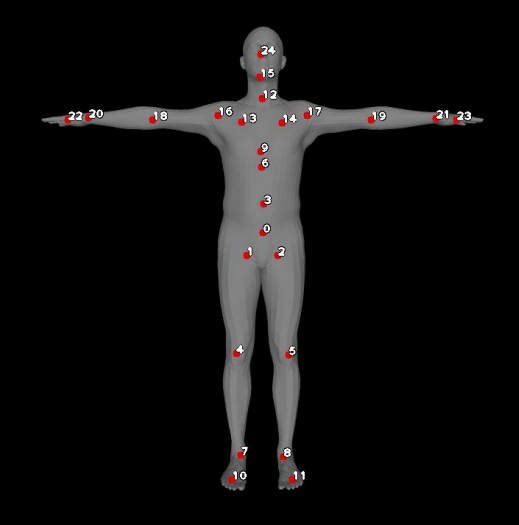
\includegraphics[width=0.5\linewidth]{images/smpl_joint_structure.png}
  \caption{An image of the position of joints in the SMPL skeleton}
  \label{fig:smpljointstructure}
\end{figure}

Looking at Figure \ref{fig:smpljointstructure} provided by \cite{smplpowerpoint}, we can use these ids to map what indices of our mocap data correlate to for DeepMimic.

\begin{table}[]
  \caption{A mapping of DeepMimic indices to SMPL indices}\label{tab:smpltodeepmimic}
  \begin{tabular}{|l|l|
    >{\columncolor[HTML]{C0C0C0}}l |
    >{\columncolor[HTML]{C0C0C0}}l |l|l|
    >{\columncolor[HTML]{C0C0C0}}l |
    >{\columncolor[HTML]{C0C0C0}}l |}
    \hline
  \cellcolor[HTML]{9B9B9B}DeepMimic & \cellcolor[HTML]{9B9B9B}i & \cellcolor[HTML]{9B9B9B}SMPL & \cellcolor[HTML]{9B9B9B}i & \cellcolor[HTML]{9B9B9B}DeepMimic & \cellcolor[HTML]{9B9B9B}i & \cellcolor[HTML]{9B9B9B}SMPL & \cellcolor[HTML]{9B9B9B}i \\
  Root                              & 1:4                       & transl                       & -                         & R\_shoulder                       & 25:29                     & R\_shoulder                  & 16                        \\
  Root rotate                       & 4:8                       & global\_orient               & 0                         & R\_elbow                          & 29                        & R\_elbow                     & 18                        \\
  Chest                             & 8:12                      & Spine3                       & 8                         & L\_hip                            & 30:34                     & L\_hip                       & 0                         \\
  Neck                              & 12:16                     & Neck                         & 11                        & L\_knee                           & 34                        & L\_knee                      & 3                         \\
  R\_hip                            & 16:20                     & R\_hip                       & 1                         & L\_ankle                          & 35:39                     & L\_ankle                     & 6                         \\
  R\_knee                           & 20                        & R\_knee                      & 4                         & L\_shoulder                       & 39:43                     & L\_shoulder                  & 15                        \\
  R\_ankle                          & 21:25                     & R\_ankle                     & 7                         & L\_elbow                          & 43                        & L\_elbow                     & 17                       
  \end{tabular}
  \end{table}

\subsection{Swapping of Axes}

The mocap data that we're provided with comes in a vector of shape (3 $\times$ 3), a rotation vector. This means that we have to convert it to quaternions, for normal joints, or axis angles, for the revolute joints.

Before this, however, we can solve the issue of difference in axis convention. For example, we could say that the DeepMimic character follows the rule of "XYZ", where the character faces towards X, Y points up, and Z points to the right. In its own program, the SMPL-X character also follows this. But we can see from \ref{fig:humanoids_in_program} that they do not face the same way. Thus, following this logic, the global orientation of the characters would correlate to different axes. Because the SMPL-X character is facing towards the left of the DeepMimic humanoid, the character's global orientation would have to be rotated around the Y axis to the clockwise. The "XYZ" of the SMPL-X character now has X facing left, and the character facing towards Z. To maintain convention, we would convert "XYZ" to "ZY(-X)". While we cannot be sure that our CHI3D dataset will have the same relevant axes, we can take this theory and extrapolate from there for our implementation. A potential issue from this line of thinking is that we are assuming that "XYZ" means that the character faces the positive direction of X, that the positive Y direction points up, and that the positive Z direction points towards the right of our character. This could be easily wrong if say, for example, the DeepMimic humanoid has the positive Z direction point towards the right of our character, but our SMPL-X character has its positive X direction point towards the left of the character. This would mean that our conversion would now have to be "XYZ" to "(-Z)Y(-X). This is hypothetical, but means that our permutations of combinations go from $3!$ to a larger number. The exact number would be $6 \times 4 \times 2 = 48$. Specifically, this is a modified version of the permutation formula. The permutation formula is defined as:
\begin{equation}
  \frac{n!}{(n-r)!}
\end{equation}
where $n!$ is the total number of permutations we can get from a set of n, and r is the number of elements we want to choose.
But in our case, when we choose an element, we also remove its corresponding negative or positive element, depending on what we chose. So our equation is actually
\begin{equation}
  \frac{n!}{O}
\end{equation}
where $O$ represents a subset of $n!$ without the multiplication of odd numbers. 48 is a lot of numbers that we can go through, so we can't reasonably be expected to trial-and-error the swapping of axes.

One hint we can think of is the transl field. The transl field is the translation of the root joint for our SMPL-X character, which correlates to the global position of the root joint in our DeepMimic humanoid. By comparing the general movement of a mocap video, we can observe how a non-edited SMPL-X character would move when imported into the format we want. For instance, due to the movement of our clips, we can be reasonably sure that our character would have the least amount of movement in the Y-axis, as our mocap clips generally do not have the subjects in them jumping or crouching. Our permutations now become $4 \times 2 = 8$, cutting our choices down significantly. Our SMPL-X mocap clips could also contain significant differences in the other axes. An example of this being if a character only moves forward, and doesn't vary movement to their side too much. So our general order would be finding a mocap clip with large movements both forwards and sideways, and distinguish our Y-axis from it. We would then find a mocap clip that only has forwards movement, and be able to discover our Z-axis.

After we get the axis order from this process, we can apply our transformation of axes to the global\_orient field, as well as the fields in body\_pose.

\subsection{Rotation of Joints}
We also have to take into account the rotation of joints, global and local. The first rotation we have to take care of is the global orientation. Making sure that our character faces the right way is imperative, and the global orientation of our root joint is the easiest one to manipulate. This is because it is a global rotation, which means that the rotation corresponds to our world coordinates.

Firstly, we have to understand rotation matrixes, as our SMPL-X mocap data comes in this rotation format for their joints. The rotation matrix for angles $\theta$ around an axis are given by the following 3 formula.

Rotation around the x-axis:
\begin{equation}
  R_x(\theta) = \begin{bmatrix}
    1 & 0 & 0\\
    0 & \cos\theta & -\sin\theta\\
    0 & \sin\theta & \cos\theta
  \end{bmatrix}
\end{equation}

Rotation around the y-axis:
\begin{equation}
  R_y(\theta) = \begin{bmatrix}
    \cos\theta & 0 & \sin\theta\\
    0 & 1 & 0\\
    -\sin\theta & 0 & \cos\theta
  \end{bmatrix}
\end{equation}

Rotation around the z-axis:
\begin{equation}
  R_y(\theta) = \begin{bmatrix}
    \cos\theta & -\sin\theta & 0\\
    \sin\theta & \cos\theta & 0\\
    0 & 0 & 1
  \end{bmatrix}
\end{equation}

Matrix representation of a rotation of a joint is given by the following formula, where X, Y, and Z are the counterclockwise rotation around their respective axes: 
{\small
\begin{equation}
  \begin{aligned}
    R & = R_z(Z)R_y(Y)R_x(X)\\
    & = \begin{bmatrix}
      \cos(Z) & -\sin(Z) & 0\\
      \sin(Z) & \cos(Z) & 0\\
      0 & 0 & 1
      \end{bmatrix}
      \begin{bmatrix}
        \cos(Y) & 0 & \sin(Y)\\
        0 & 1 & 0\\
        -\sin(Y) & 0 & \cos(Y)
      \end{bmatrix}
      \begin{bmatrix}
        1 & 0 & 0\\
        0 & \cos(X) & -\sin(X)\\
        0 & \sin(X) & \cos(X)
      \end{bmatrix}\\
    & = \begin{bmatrix}
        \cos(Y)\cos(Z) & \sin(X)\sin(Y)\cos(Z)-\cos(X)\sin(Z) & \cos(X)\sin(Y)\cos(Z)+\sin(X)\sin(Z)\\
        \cos(Y)\sin(Z) & \sin(X)\sin(Y)\sin(Z)+\cos(X)\cos(Z) & \cos(X)\sin(Y)\sin(Z)-\sin(X)\cos(Z)\\
        -\sin(Y) & \sin(X)\cos(Y) & \cos(X)\cos(Y)
      \end{bmatrix}
  \end{aligned}
\end{equation}
}

Multiplying these rotations together using matrix multiplication in a specific order is what gives us our original rotation matrixes. Rotation matrixes are hard to manage, however, and not good for our conversion. If we rotated around an axis, the rotation would also affect other axes due to the way rotation matrixes are. Rotation matrixes have the issue of running into gimbal locks, which is the loss of one degree of freedom at certain alignment of the axes. For our $(3\times3)$ matrix, when 2 axes are parallel, the rotation turns into a two-dimensional space. Matrix multiplication is not commutative, so the order in which rotations are performed has to be specified. Rotation matrixes are more for applying a shift of axes to a column or row vector. 

Since rotation matrixes are hard to manage, we could change this by converting our rotation matrixes to quaternions. This also works to our advantage as we need the quaternion format for DeepMimic.

Quaternions are a way of representing rotations of elements in a three dimensional space, by rotating about an arbitrary axis. They're commonly used in the 3d graphics area, due to their reliablity and usefullness. Quaternions are more compact as a format of (4), and simpler than rotation matrixes. They also don't suffer from gimbal locks. Quaternions are also not commutative. The reason why quaternions are a shape of 4 elements is because it consists of one real part and 3 imaginary parts.

The format we want for DeepMimic is (w,x,y,z), where w is the real scalar number, while x,y,z are imaginary vectors.

The general formula for a quaternion is:

\begin{equation}
  q = w + xi + yj +zk
\end{equation}

So, to get our given rotations, we get:

\begin{equation}
  \begin{aligned}
    w &= \cos\frac{\theta}{2}\\
    x &= i\times\sin\frac{\theta}{2}\\
    y &= j\times\sin\frac{\theta}{2}\\
    z &= k\times\sin\frac{\theta}{2}
  \end{aligned}
\end{equation}
where i,j,k are equivalent to unit vectors on their axes. Theta is represented in radians We can get the rotations we want by creating another quaternion from a unit vector, and multiplying both quaternions for the final product we want. Note that the multiplication is not commutative. For example, rotating a joint about the Y-axis for $90^{\circ}$ and then about the Z-axis is not the same as rotating it about the Z axis and then the Y-axis.

Taking our root orientation into account, if we say that the SMPL-X character needs to be rotated $90^{\circ}$ clockwise around the y-axis, we would get a rotation quaternion of:

\begin{equation}
  \begin{aligned}
    w_2 = (\cos\frac{frac{\pi}{2}}{2})
    x_2 = 0
    y_2 = -\sin\frac{\frac{\pi}{2}}{2}
    z_2 = 0
\end{aligned}
\end{equation}

We would then multiply the original quaternion $q_1 = (w_1, x_1, y_1, z_1)$ by this quaternion, $q_2$.

\begin{equation}
  \begin{aligned}
    w_3 = w_1w_2 - x_1x_2 - y_1y_2 - z_1z_2\\
    x_3 = w_1x_2 + x_1w_2 + y_1z_2 - z_1y_2\\
    y_3 = w_1y_2 - x_1z_2 + y_1w_2 + z_1x_2\\
    z_3 = w_1z_2 + x_1y_2 - y_1x_2 + z_1w_2\\
  \end{aligned}
\end{equation}

We need to do this for the root orientation, as well as the joints at the shoulders in order to bring them down into the default position of the humanoid. For example, if the SMPL-X charactr is facing towards the X-axis, we would need to rotate around the x-axis and bring the arm down. However, since the rotation of arms is already present in the mocap data, we would need to account for this, as since the multiplication is not commutative, simply applying a rotation to bring the arms down would not work.

Another method of going about it would be creating a copy of the DeepMimic humanoid, but this time in a T-Pose. This way, we avoid the commutative issues.

We also have to be concerned about the revolute joints. As a dimension of 1, the revolute joints of the DeepMimic humanoid are unique, as SMPL-X does not take them as revolute joints and has them on the same $(3\times3)$ rotation matrix. We can solve this by potentially converting them to quaternions and calculating the magnitude of the scalar change, and isolating it to become our revolute rotation. We do this by using the w real angle, and using its formula to find $\theta$.

\begin{equation}
  \begin{aligned}
    w &= \cos\frac{\theta}{2}\\
    \arccos (w) &=\frac{\theta}{2}\\
    2\arccos (w) &=\theta\\
  \end{aligned}
\end{equation}
\clearpage
\section{Changing DeepMimic to implement Multiple Characters}
To change the DeepMimic program to implement multiple characters, we can first address the issues of the arguments. Documentation will have to be created so that the user knows what arguments they can use. Additionally, we need to implement a proper way to generate a character at a fixed location. Otherwise, the characters will spawn at the root of the world, in the same place, and collide, instantly causing the characters to fail their motion.

We then need to fix the source code not accounting for the addition of multiple characters. A good way to keep track of this would be to draw a map of classes that make use of one another.

\subsection{A program to generate a argument file}
Another idea I had for the argument file would be to create a program that would prompt the user, asking what kind of scene they would like to create, and then going more into detail about the arguments by giving the argument field and valid answers, and then asking the user what value they would like to input. This then produces an argument file that you can use to run DeepMimic scenes.

\subsection{A Map of the Files needed to Implement Multiple Characters}

To see the list of changes needed to be made, a diagram of the general system design would be very helpful. Figure \ref{fig:classdiagram} keeps track of what is needed to be changed, and if any errors occur, is useful to refer back to.

\begin{figure}[htb]
  \centering
  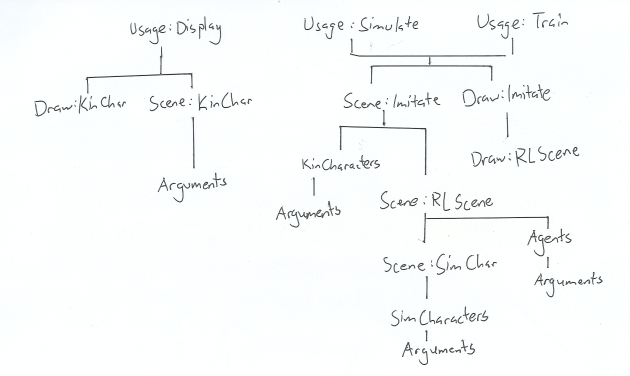
\includegraphics[width=1.0\linewidth]{images/class_structure.png}
  \caption{A diagram of what a user will be interacting with in this paper, and the relevant areas that need to be changed to accomodate multiple characters}
  \label{fig:classdiagram}
\end{figure}

%==================================================================================================================================
\chapter{Implementation}
After the analysis of what issues DeepMimic has, we designed solutions attempting to address them.

\section{Conversion}
For the conversion of CHI3D datasets, I chose to use Python. We can use the pytorch libary to reduce risk of errors of our own conversion from matrices to quaternions, as they already have preexisting functions to automate our conversion.

However, we have to make our own rotation functions. I chose to have a rotate\_x, rotate\_y and rotate\_z function, which takes a parameter of angles in degrees and converts it to radians, before multiplying the original rotation with it. To implement this, the library of numpy is versatile and helps in making the correct vectors that I need.

A Python file takes in the CHI3D mocap file, with parameters such as input and output paths, frame per second, and whether movement should be a loop or not. The field to change these parameters is on top so the user has easy access to change them at will. Frames per second also converts to its necessary frame time, which is given by $\frac{1}{T}$, T being the frames per second. Using indexing, I mapped the converted file as per the diagram above to their relevant bones. Then I output the result, which is a DeepMimic format mocap file.

I also wrote a function that would change the axes of the rotations, with parameters for simple notations. If a user wanted to convert "XYZ" to "YX(-Z)", they could specify it in the parameters using strings. The function will then change the axes of the motion accordingly.

Loading in some mocap files from CHI3D, for example Grab\_2, I saw that for the "XYZ" of SMPL-X, Y was moving too much. Additionally, the character spawned in the ground as a result. Y is not the same as Y for DeepMimic. Trying the X field, by swapping the axes around also lacked results, as the character continued to rise and fall. However, the Z axis seemed to be stationary, which meant that I found the corresponding Y. I then checked to see whether this held true for the global rotation. Going from the previous diagram, I tried rotating the character 90 degrees around the Y-axis clockwise.

However, while I did get the characters to rotate and face the same way eventually, I tried to convert the dataset by rotating the shoulders 90 degrees down. This did not work, meaning that my hypothesis that the non-commutative nature of the rotation multiplication held true. Unless I wanted to fine tune every rotation for every frame, that was not going to be a viable option.

In the end, I ended up having to make another python file, which took DeepMimic motion files, and globally rotated them around the y-Axis, and made the movement of the x-axis and z-axis negative. This was so I could flip the movement of whatever file I used. My reasoning behind this was that if I wanted the two characters to interact with each other, I could not have them both moving the same way, and instead wanted them to move towards each other, hence the flipped movement. The file I used was a file that made a character step forward and punch. This at least fulfilled the requirements of two characters interacting with each other, as I could use them to punch each other. Another reason I chose punch was because it was not a looped motion file, which was perfect for the purposes of my study. While this was still operating under the mistake of non-commutative multiplication, from checking the display to see how the character moved, I noticed that the motion did not change that much, and the character's ending position for their foot slightly clipped into the ground. This was fine for my purposes, so I used it.

\section{Argument Parsing}
For argument parsing, I made the arguments for the usage of display and simulation consistent. This involved making sure display accepted the simulation argument of "character\_files", instead of a singular "character\_file" in its argument. Keeping the same convention is important so as to not confuse the user. I then went through the arguments parsers, where I made all relevant arguments accept an array of the objects they were supposed to receive. This was meant to prepare for the implementation of multiple characters.

For users who do want to edit the argument files, I have prepared the relevant documentation for them in Table \ref{tab:arguments}. This documentation comes in this dissertation, in the appendix, which contains the same structure as the argument file making, splitting them up in a logical way. In the document, arguments and their respective valid inputs are given.

\section{Display}
My first attempt at making multiple characters function was to display two characters at once. Logically, this is the easiest one to do, as it only involves one scene. At this time, I was relatively inexperienced in C++, so I struggled with adapting the pre-existing source code. However, I was able to find a fork request from Github user Yiziki\footnote{\url{https://github.com/xbpeng/DeepMimic/pull/199}}, which had attempted to implement the display of multiple characters as well. Their implementation did not work, but was useful in providing the syntax and classes that I needed to focus on. They also had trouble with their argument files, leading to segmentation faults, which is partially why their implementation did not work. I edited my clone of the DeepMimic repository and fixed the relevant functions, being related to argument parsing, character initialisation, and drawing of the characters, along with the functions that involved fetching a character by id. These functions had to be overloaded as I was unsure if any other functions would use the non-overloaded ones, but I changed the majority of retrievals to use the id parameter.

As a design choice, I did not implement a way to edit the initial position of the characters in Scene Kin Char. This is because my initial issues with position initialisation were due to the characters colliding and not being able to perform their function. Simulation would also be where I wanted to make two characters interact, so initial positions were important there. For just displaying a motion, this was not needed.

\section{Simulation}
By this time, I was more experienced in C++ now and knew what had to be done. The choice to start with Display first meant that the update for the more important simulation scenes would be better implemented. As with SceneKinChar, SceneImitate needed functions that initialised characters to be changed, and variables that were meant to house a single character would need to be extended into an array. An example of this is the mKinChar field, which used to hold just one KinChar character. With the array, it could now hold multiple characters. The same GetCharacter functions were also changed to accept ids.

I ran into an issue where two characters were initialised, but were not moving and reacting to the motion files provided. This turned out to be a controller issue, where the respective KinControllers were not being assigned to the proper KinChars. Syncing the KinChars and SimChars had to be edited as well, to fix this.

Once fixed, characters were displaying properly. To test, I used two different motion files that Peng provided so they would not intefere with the other character's motion as much. I did this by selecting the movement of jump and roll, which had the least overlap, particularly because roll had a different y position to jump.

After the simulation of multiple characters could be achieved, the problem of the initialisation of starting position for characters needed to be solved. First, the argument for the random character position was enabled, but changed nothing. After looking through the code, it became apparent that random character position didn't actually do anything. It just set the character's position to the root of the world again, as shown in Listing \ref{lst:randomisation}. The only thing the random placement calculates is a vector filled with zeros, which doesn't move the character at all.

\begin{lstlisting}[language=C++, float, caption={The function related to character position randomisation}, label=lst:randomisation]
  void cSceneSimChar::SetCharRandPlacement(const std::shared_ptr<cSimCharacter>& out_char)
  {
    tVector rand_pos = tVector::Zero();
    tQuaternion rand_rot = tQuaternion::Identity();
    CalcCharRandPlacement(out_char, rand_pos, rand_rot);
    out_char->SetRootTransform(rand_pos, rand_rot);
  }

  void cSceneSimChar::CalcCharRandPlacement(const std::shared_ptr<cSimCharacter>& out_char, tVector& out_pos, tQuaternion& out_rot)
  {
    tVector char_pos = out_char->GetRootPos();
    tQuaternion char_rot = out_char->GetRootRotation();

    tVector rand_pos;
    tQuaternion rand_rot;
    mGround->SamplePlacement(tVector::Zero(), rand_pos, rand_rot);

    out_pos = rand_pos;
    out_pos[1] += char_pos[1];
    out_rot = rand_rot * char_rot;
  }

\end{lstlisting}

This was fixed through the calling for a random number, and adding it to the position of the character's original position. Initially, this was only a randomisation of the x-axis.

After confirming that the random variable finally worked, I began working on fixed position offsetting. There is already an argument for this, that shifts a character's position along the x-axis by parsing a double. There was no way to randomise the z-axis, however, as the parameters only cared about changing the x-axis. This was an easy fix, and now the characters are ready to be moved around the plane of the world.

User adjusted character offset for random placements was also implemented, by adding the user's arguments to the character's root position, and then adding or subtracting a random magnitude from the x-axis or z-axis. The y-axis was left unrandomised as I felt it wasn't worth implementing, due to the focus being on the interaction of two characters. Randomising y values might just lead to poor results, and doesn't contribute anything to the overall project.

\subsection{Training of Policies}
Once the Imitate scene is finished, I started working on training policies. Firstly, I trained a movement dataset that had been flipped around. This involved training a character solo, to make sure it could stand on its own. If I had to stop the training at any time, I used the argument to select a pre-existing policy and selected the previous outputted policy. This is a workaround to the lack of being able to pause and resume training, in case I needed to work on other aspects of the program or restart my hardware. After a combined sixty-million samples, which is what is suggested, I then started to train two characters at once.

I used the policy that was made during the solo training of our inversed puncher and put two characters in a scene together, with a fixed position. One character used the inversed policy, and the other, the normal policy. I judged the position myself by slowly increasing the offset values until they were interacting in a way that I wanted them to. My criteria for this was that they had to be far enough to not completely collide into each other before completing their motion, but close enough such that the edges of their motion still collided with each other.

Looking through the logs of the policies that were trained, I saw that they were quite hard to read. I decided to write a script in python that converted the last outcome of the logs to be more presentable.

%==================================================================================================================================
\chapter{Evaluation}

\section{Evaluation of Work Done}
\subsection{Conversion}
Unforetunately, I was unable to get the conversion finished. The initial idea I made, rotation about an axis applied to the joints, was flawed as it did not take into account the non-commutative aspect of rotations. As the data set already has a rotation, the axes would have already changed, which means that if I wanted to make the dataset work with DeepMimic, I would need to slowly fine-tune every individual rotation in every individual frame. At that point, it becomes more work than even keyframe animation, which would defeat the whole purpose of trying to get an automated adaptable animation.

As it stands, I cut my losses and instead worked on the movements that were already inside DeepMimic. Using this, I am still able to simulate characters interacting with each other, even if these characters come from solo movements. The goal of the study is to get DeepMimic working with multiple characters, and the additional datasets come with more movements to train on, possibly more intricate. However, when weighed on cost to benefit, it is important to reprioritise goals.

\subsection{Randomisation}
The reason why the random character placement is important is because the goal of this study is to see if a character can learn to interact with another character, and perform those actions even if their environment changes. An environmental change could be something like a character shifted slightly out of position. While this can also be achieved through the fixed position, using random character placement means that a bias of trying to get good results by putting characters in only good positions can be avoided. It can also help to automate testing, where instead of changing the numbers of a fixed position minutely, the random character positions can just be called again, which saves time. The way the implementation of this was done also reflects the original goal in mind. Instead of a completely random initialisation, the root position of the character is still taken into account. It is from there that minute changes can be made, which is the randomised part, giving a repeatable action that doesn't take any fine-tuning perfectly usable for testing whether a policy holds up.

\subsection{Argument Files}
The standardisation of argument files was only made for Scene Imitate and Scene Kin Char. There are still many other scenes that have discrepancies in their argument files, but for the purpose of this research, the goals achieved were what needed to be focused on.

Additionally, the documentation solves a lot of issues I had with having to scrounge around. Documentation for programs in this day and age is very important, as it is important for anyone to be able to read through your code and distinguish what it is doing, or how they should interact with it. The documentation I wrote is made only for this project in mind, though, which means that it is focused on three things that the user would want, that being display, simulation, and training. While this layout for the documentation does make sense from a logical and convenient standpoint, it might also obfuscate some argument someone is trying to find when they do not have the same purpose as what I have achieved.
\pagebreak
\subsection{Being Able to Make Multiple Characters Interact}
The program works, and we are able to simulate and make characters interact. The more a policy is run for solo characters, the more likely that a character's movement will be successful. This also holds true when training two characters. We can see that as the program reaches more samples, the train\_return value slowly increases, and so does the test\_return. Something that might confuse the results is the lack of ability to pause and resume the training, as trying the workaround to do so tends to lower the train\_return field for a while. This is seen in Figure \ref{fig:punchconvertoutput}, which had to resume training.

\begin{figure}
  \centering
  \begin{subfigure}[b]{0.45\textwidth}
    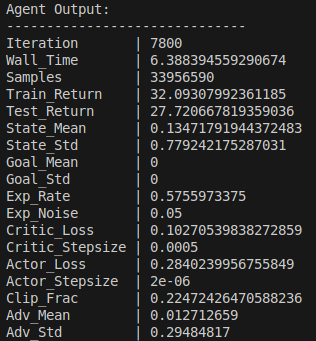
\includegraphics[width=\textwidth]{images/punch_convert_output.png}
    \caption{An output from DeepMimic, showing the statistics of the earliest run of training Punch Convert}
    \label{fig:punchconvertoutput1}
  \end{subfigure}
  \begin{subfigure}[b]{0.45\textwidth}
    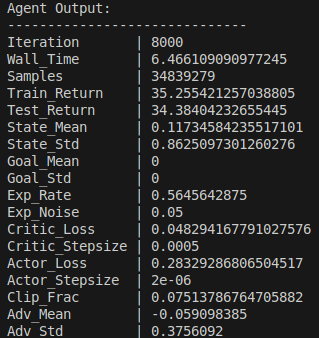
\includegraphics[width=\textwidth]{images/punch_convert_output_2.png}
    \caption{An output from DeepMimic, showing the statistics of the later run of training Punch Convert}
    \label{fig:punchconvertoutput2}
  \end{subfigure}
  \caption{Outputs from DeepMimic, showing policy training on the solo conversion of the punch movement that was flipped about the y axis}
  \label{fig:punchconvertoutput}
\end{figure}

The training of the multiple characters interacting went well. Each iteration returned a larger train and test return number, which showed that both models were increasingly learning. This is seen in the difference of results in Figure \ref{fig:earlymultipletrainingresults} and \ref{fig:multipletrainingresults}, where there is a difference of train return, that being $30.2-13.5=16.7$, and a difference in test return, being $26.4-19.9=6.5$. The huge jump in successful returns is probably related to the huge difference in samples, with the earlier run only having 7589798 samples, and the later model having that number plus its own, $7589798+52632477=60222275$. This number is the bare minimum that Peng said would give consistent results to simple movements.

\begin{figure}
  \begin{subfigure}[b]{0.45\textwidth}
    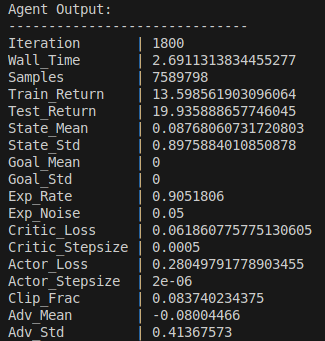
\includegraphics[width=\textwidth]{images/multiple_agent0_1.png}
    \caption{An output from DeepMimic, showing the statistics of Agent0}
    \label{fig:earlymultipletrainingresults1}
  \end{subfigure}
  \begin{subfigure}[b]{0.45\textwidth}
    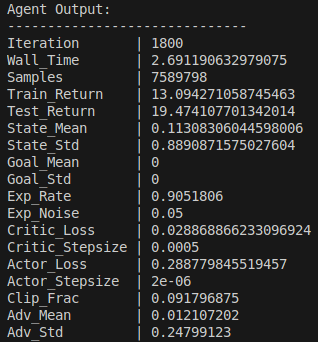
\includegraphics[width=\textwidth]{images/multiple_agent1_1.png}
    \caption{An output from DeepMimic, showing the statistics of Agent1}
    \label{fig:earlymultipletrainingresults2}
  \end{subfigure}
  \caption{Outputs from DeepMimic, showing an earlier run of policy training on multiple characters interacting with each other}
  \label{fig:earlymultipletrainingresults}
\end{figure}

\begin{figure}
  \begin{subfigure}[b]{0.45\textwidth}
    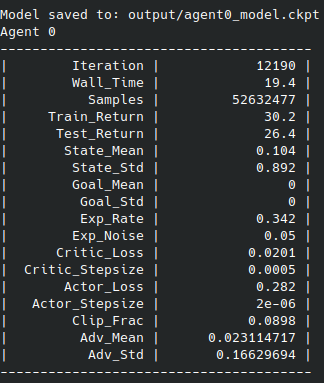
\includegraphics[width=\textwidth]{images/agent0_later_training.png}
    \caption{An output from DeepMimic, showing the statistics of Agent0}
    \label{fig:multipletrainingresults1}
  \end{subfigure}
  \begin{subfigure}[b]{0.45\textwidth}
    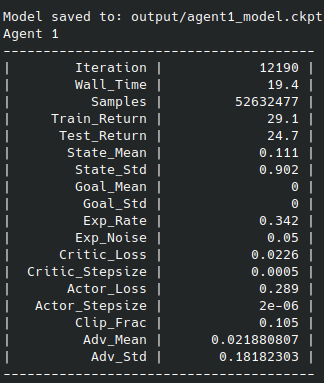
\includegraphics[width=\textwidth]{images/agent1_later_training.png}
    \caption{An output from DeepMimic, showing the statistics of Agent1}
    \label{fig:multipletrainingresults2}
  \end{subfigure}
  \caption{Outputs from DeepMimic, showing the last policy training on the multiple characters of the punch movement}
  \label{fig:multipletrainingresults}
\end{figure}

In Figure \ref{fig:picturedinteraction}, we see the difference in policies trained. When learning on their own, the characters miss each other completely, which is not a desired outcome. However, the characters that learned together are able to punch each other and still retain a consistent movement. The difference in outcomes here show that my implementation works, and delivers more consistent results than programs that would just train their own characters solitarily.

\begin{figure}
  \begin{subfigure}[b]{0.45\textwidth}
    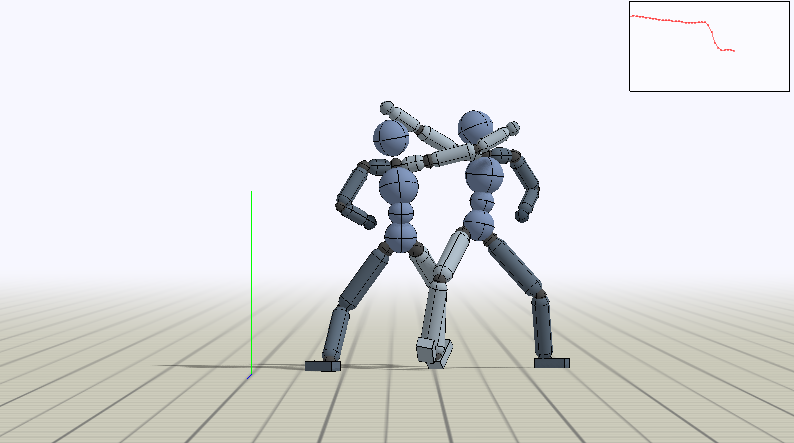
\includegraphics[width=\textwidth]{images/interaction_fail.png}
    \caption{The simulation of policies that used the individual characters learning on their own}
    \label{fig:interactionfail}
  \end{subfigure}
  \begin{subfigure}[b]{0.45\textwidth}
    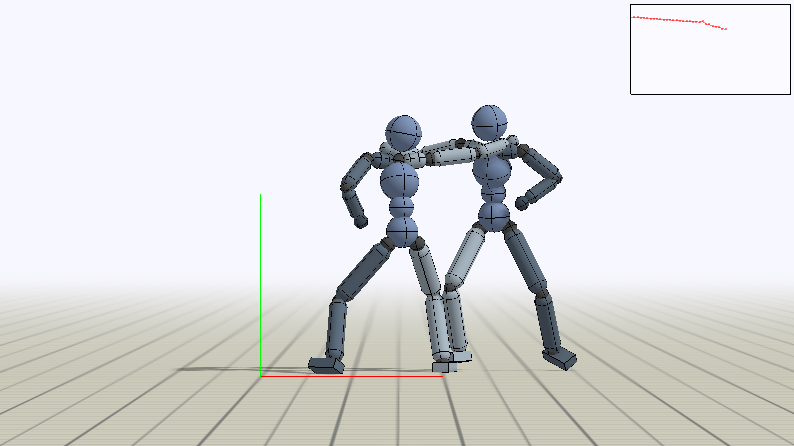
\includegraphics[width=\textwidth]{images/interaction.png}
    \caption{The simulation of policies that had the characters learning together}
    \label{fig:interactionsucceed}
  \end{subfigure}
  \caption{DeepMimic running simulations on multiple characters. The graph in the upper-right tracks the success of the movement of the character. The lower it goes, the poorer the character performed.}
  \label{fig:picturedinteraction}
\end{figure}

Due to the nature of this program, possible difficulties arise. One such issue is the training of multiple characters at once. The code calls for a reset of the scene if a character falls down. This means that no matter which character falls, the controllers are reset, and the agent decides that the movement was a failure and marks it down as such. This doesn't take into account the circumstance of one character failing and the other one succeeding. Because one character fails, the other character also marks it as a negative outcome even if their motion was about to succeed, creating a false negative, and thus what the character learns would be wrong.

Another issue that arises it definitely the long amount of time that the program takes to run. To properly train a simple policy, \cite{deepmimic} describes how it takes almost a day, sixty million samples roughly. When we factor in another character, this makes the movement much more complicated, and thus more samples would need to be generated, leading to higher run times. If we naively assume that adding on another character would double the amount of samples needed, that means that the program would take two days to run, which is not ideal.

%==================================================================================================================================
\chapter{Conclusion}    

\section{Recap}
In summary, the world is in a place where virtual environments are becoming more advanced and commonplace. It's a billion-dollar industry that only seems to be increasing in advancements. Physics-based character animation is a very adaptable and cost-effective way of character animation, compared to other, more traditional methods. When we introduce Deep Reinforcement learning, we are able to push this even further. By expanding the scope of these programs to incorporate intricate interactions between characters, we make a future in which animation is no longer as costly, where animators are less overworked, where technology becomes even more realistic. I was able to implement the ability to use programs like these to attempt to train character interactions, albeit naively. Future work could expand on this by using this program to start training interactions between video game characters, where terrains are uneven and completely unique. They could use this to simulate new movements for robotic characters, use that data to program in automated movement, to enable them to walk around a real life environment. We can even use this research to supplement old methods. For example, we could supplement keyframe animation by making the frames in between use our policies, thus making the animation both realistic and stylised when it needs to be. By making reinforcement learning physics-based character animation the norm, we would be able to push the animation industry forward towards a new revolution.

\section{Reflection}
What went well was the implementation of multiple characters. Now that I am more familiar with the source code and C++ as a whole, I feel more confident in my ability to continue working on this. My expanded knowledge on rotation joints and the format they come in would also come in handy.

If I had the chance to work on this again, knowing what I know now, I would have focused on creating a humanoid with the same default posture as the outside mocap data skeletons. This would probably have been a better solution than attempting to rotate the already captured motion data. The conversion script would probably work then, and that would have left me with a bigger amount of movements to train.

\section{Future Work}
To take this further, I would like to see what happens when training character interactions, but with a bigger reward factor based on a specific joint reaching a goal. For example, let us take two characters shaking hands. The focus and key here would be the locking of hands, the characters being able to touch one another. This would be affected by something like the scale of a character. If we were to leave one character at the same scale, but lower the height of another character, their hands would miss each other completely. Technically, they would still complete their movement, but the context and meaning behind the interaction is lost. To solve this, I imagine I could place some emphasis on the reward value of their hand joints reaching a specific coordinate or touching each other. It's like placing more weight behind the outcome of that specific joint achieving its goal.

%==================================================================================================================================
%
% 
%==================================================================================================================================
%  APPENDICES  

\begin{appendices}

\chapter{Appendices}

\begin{itemize}
\item
\begin{table}[ht]
  \centering
  \caption{The arguments important to this project. A label of 1 means only 1 argument is needed, and M relates to the amount of characters wanted.}\label{tab:arguments}
  \begin{adjustbox}{width=1\textwidth}
  \small
  \begin{tabular}{|ll
  >{\columncolor[HTML]{C0C0C0}}l |ll
  >{\columncolor[HTML]{C0C0C0}}l |ll
  >{\columncolor[HTML]{C0C0C0}}l |}
  \hline
  \multicolumn{3}{|l|}{\cellcolor[HTML]{9B9B9B}For Display}                                        & \multicolumn{3}{l|}{\cellcolor[HTML]{9B9B9B}For Simulation}                                                                     & \multicolumn{3}{l|}{\cellcolor[HTML]{9B9B9B}For Training}                                                                                    \\ \hline
  \multicolumn{1}{|l|}{scene}            & \multicolumn{1}{l|}{kin\_char}                      &   & \multicolumn{1}{l|}{scene}                         & \multicolumn{1}{l|}{imitate}                                           &   & \multicolumn{1}{l|}{scene}                       & \multicolumn{1}{l|}{imitate}                                                          &   \\ \hline
  \multicolumn{1}{|l|}{character\_files} & \multicolumn{1}{l|}{data/characters/humanoid3d.txt} & M & \multicolumn{1}{l|}{enable\_rand\_char\_placement} & \multicolumn{1}{l|}{boolean true/false}                                & 1 & \multicolumn{1}{l|}{time\_lim\_min}              & \multicolumn{1}{l|}{0.5}                                                              & 1 \\ \hline
  \multicolumn{1}{|l|}{kin\_ctrl}        & \multicolumn{1}{l|}{motion}                         & 1 & \multicolumn{1}{l|}{num\_update\_substeps}         & \multicolumn{1}{l|}{10}                                                & 1 & \multicolumn{1}{l|}{time\_lim\_max}              & \multicolumn{1}{l|}{0.5}                                                              & 1 \\ \hline
  \multicolumn{1}{|l|}{motion\_files}    & \multicolumn{1}{l|}{path to motion file}            & M & \multicolumn{1}{l|}{world\_scale}                  & \multicolumn{1}{l|}{4}                                                 & 1 & \multicolumn{1}{l|}{time\_lim\_exp}              & \multicolumn{1}{l|}{0.2}                                                              & 1 \\ \hline
  \multicolumn{1}{|l|}{}                 & \multicolumn{1}{l|}{}                               &   & \multicolumn{1}{l|}{terrain\_file}                 & \multicolumn{1}{l|}{data/terrain/plane.txt}                            & 1 & \multicolumn{1}{l|}{time\_end\_lim\_min}         & \multicolumn{1}{l|}{20}                                                               & 1 \\ \hline
  \multicolumn{1}{|l|}{}                 & \multicolumn{1}{l|}{}                               &   & \multicolumn{1}{l|}{char\_types}                   & \multicolumn{1}{l|}{general}                                           & 1 & \multicolumn{1}{l|}{time\_end\_lim\_max}         & \multicolumn{1}{l|}{20}                                                               & 1 \\ \hline
  \multicolumn{1}{|l|}{}                 & \multicolumn{1}{l|}{}                               &   & \multicolumn{1}{l|}{character\_files}              & \multicolumn{1}{l|}{data/characters/humanoid3d.txt}                    & M & \multicolumn{1}{l|}{time\_end\_lim\_max}         & \multicolumn{1}{l|}{50}                                                               & 1 \\ \hline
  \multicolumn{1}{|l|}{}                 & \multicolumn{1}{l|}{}                               &   & \multicolumn{1}{l|}{char\_init\_pos\_xs}           & \multicolumn{1}{l|}{double (e.g. 0.0)}                                 & M & \multicolumn{1}{l|}{time\_end\_lim\_exp}         & \multicolumn{1}{l|}{50}                                                               & 1 \\ \hline
  \multicolumn{1}{|l|}{}                 & \multicolumn{1}{l|}{}                               &   & \multicolumn{1}{l|}{char\_init\_pos\_zs}           & \multicolumn{1}{l|}{double (e.g. 0.0)}                                 & M & \multicolumn{1}{l|}{anneal\_samples}             & \multicolumn{1}{l|}{32000000}                                                         & 1 \\ \hline
  \multicolumn{1}{|l|}{}                 & \multicolumn{1}{l|}{}                               &   & \multicolumn{1}{l|}{enable\_char\_soft\_contact}   & \multicolumn{1}{l|}{false}                                             & 1 & \multicolumn{1}{l|}{num\_update\_substeps}       & \multicolumn{1}{l|}{10}                                                               & 1 \\ \hline
  \multicolumn{1}{|l|}{}                 & \multicolumn{1}{l|}{}                               &   & \multicolumn{1}{l|}{fall\_contact\_bodies}         & \multicolumn{1}{l|}{0 1 2 3 4 6 7 8 9 10 12 13 14}                     & 1 & \multicolumn{1}{l|}{num\_sim\_substeps}          & \multicolumn{1}{l|}{2}                                                                & 1 \\ \hline
  \multicolumn{1}{|l|}{}                 & \multicolumn{1}{l|}{}                               &   & \multicolumn{1}{l|}{char\_ctrls}                   & \multicolumn{1}{l|}{ct\_pd}                                            & M & \multicolumn{1}{l|}{world\_scale}                & \multicolumn{1}{l|}{4}                                                                & 1 \\ \hline
  \multicolumn{1}{|l|}{}                 & \multicolumn{1}{l|}{}                               &   & \multicolumn{1}{l|}{char\_ctrl\_files}             & \multicolumn{1}{l|}{data/controllers/humanoid3d\_phase\_rot\_ctrl.txt} & M & \multicolumn{1}{l|}{terrain\_file}               & \multicolumn{1}{l|}{data/terrain/plane.txt}                                           & 1 \\ \hline
  \multicolumn{1}{|l|}{}                 & \multicolumn{1}{l|}{}                               &   & \multicolumn{1}{l|}{kin\_ctrl}                     & \multicolumn{1}{l|}{motion}                                            & 1 & \multicolumn{1}{l|}{char\_types}                 & \multicolumn{1}{l|}{general}                                                          & 1 \\ \hline
  \multicolumn{1}{|l|}{}                 & \multicolumn{1}{l|}{}                               &   & \multicolumn{1}{l|}{motion\_files}                 & \multicolumn{1}{l|}{path to motion file}                               & M & \multicolumn{1}{l|}{character\_files}            & \multicolumn{1}{l|}{data/characters/humanoid3d.txt}                                   & M \\ \hline
  \multicolumn{1}{|l|}{}                 & \multicolumn{1}{l|}{}                               &   & \multicolumn{1}{l|}{sync\_char\_root\_pos}         & \multicolumn{1}{l|}{true}                                              & 1 & \multicolumn{1}{l|}{char\_init\_pos\_xs}         & \multicolumn{1}{l|}{double}                                                           & M \\ \hline
  \multicolumn{1}{|l|}{}                 & \multicolumn{1}{l|}{}                               &   & \multicolumn{1}{l|}{sync\_char\_root\_rot}         & \multicolumn{1}{l|}{false}                                             & 1 & \multicolumn{1}{l|}{char\_init\_pos\_zs}         & \multicolumn{1}{l|}{double}                                                           & M \\ \hline
  \multicolumn{1}{|l|}{}                 & \multicolumn{1}{l|}{}                               &   & \multicolumn{1}{l|}{agent\_files}                  & \multicolumn{1}{l|}{data/agents/ct\_agent\_humanoid\_ppo.txt}          & M & \multicolumn{1}{l|}{enable\_char\_soft\_contact} & \multicolumn{1}{l|}{false}                                                            & 1 \\ \hline
  \multicolumn{1}{|l|}{}                 & \multicolumn{1}{l|}{}                               &   & \multicolumn{1}{l|}{train\_agents}                 & \multicolumn{1}{l|}{boolean true/false}                                & M & \multicolumn{1}{l|}{fall\_contact\_bodies}       & \multicolumn{1}{l|}{0 1 2 3 4 6 7 8 9 10 12 13 14}                                    & 1 \\ \hline
  \multicolumn{1}{|l|}{}                 & \multicolumn{1}{l|}{}                               &   & \multicolumn{1}{l|}{model\_files}                  & \multicolumn{1}{l|}{path to model files}                               & M & \multicolumn{1}{l|}{char\_ctrls}                 & \multicolumn{1}{l|}{ct\_pd}                                                           & M \\ \hline
  \multicolumn{1}{|l|}{}                 & \multicolumn{1}{l|}{}                               &   & \multicolumn{1}{l|}{}                              & \multicolumn{1}{l|}{}                                                  &   & \multicolumn{1}{l|}{char\_ctrl\_files}           & \multicolumn{1}{l|}{data/controllers/humanoid3d\_phase\_rot\_ctrl.txt}                & M \\ \hline
  \multicolumn{1}{|l|}{}                 & \multicolumn{1}{l|}{}                               &   & \multicolumn{1}{l|}{}                              & \multicolumn{1}{l|}{}                                                  &   & \multicolumn{1}{l|}{kin\_ctrl}                   & \multicolumn{1}{l|}{motion}                                                           & 1 \\ \hline
  \multicolumn{1}{|l|}{}                 & \multicolumn{1}{l|}{}                               &   & \multicolumn{1}{l|}{}                              & \multicolumn{1}{l|}{}                                                  &   & \multicolumn{1}{l|}{motion\_files}               & \multicolumn{1}{l|}{path to motion file}                                              & M \\ \hline
  \multicolumn{1}{|l|}{}                 & \multicolumn{1}{l|}{}                               &   & \multicolumn{1}{l|}{}                              & \multicolumn{1}{l|}{}                                                  &   & \multicolumn{1}{l|}{sync\_char\_root\_pos}       & \multicolumn{1}{l|}{true}                                                             & 1 \\ \hline
  \multicolumn{1}{|l|}{}                 & \multicolumn{1}{l|}{}                               &   & \multicolumn{1}{l|}{}                              & \multicolumn{1}{l|}{}                                                  &   & \multicolumn{1}{l|}{sync\_char\_root\_rot}       & \multicolumn{1}{l|}{false}                                                            & 1 \\ \hline
  \multicolumn{1}{|l|}{}                 & \multicolumn{1}{l|}{}                               &   & \multicolumn{1}{l|}{}                              & \multicolumn{1}{l|}{}                                                  &   & \multicolumn{1}{l|}{agent\_files}                & \multicolumn{1}{l|}{data/agents/ct\_agent\_humanoid\_ppo.txt}                         & M \\ \hline
  \multicolumn{1}{|l|}{}                 & \multicolumn{1}{l|}{}                               &   & \multicolumn{1}{l|}{}                              & \multicolumn{1}{l|}{}                                                  &   & \multicolumn{1}{l|}{model\_files}                & \multicolumn{1}{l|}{in case you want to resume training, if not remove from arg file} & M \\ \hline
  \multicolumn{1}{|l|}{}                 & \multicolumn{1}{l|}{}                               &   & \multicolumn{1}{l|}{}                              & \multicolumn{1}{l|}{}                                                  &   & \multicolumn{1}{l|}{output\_path}                & \multicolumn{1}{l|}{output}                                                           & 1 \\ \hline
  \end{tabular}
  \end{adjustbox}
  \end{table}
\item
Install dependencies for DeepMimic and Python, run the make file for DeepMimicCore Dependencies are found in the readme in the github.

Then you can run argument files using the commands given. The readme is also in the MultiDeepMimic base folder.

\end{itemize}

\end{appendices}

%==================================================================================================================================
%   BIBLIOGRAPHY   

% The bibliography style is agsm (Harvard)
% The bibliography always appears last, after the appendices.

\bibliographystyle{agsm}

% Force the bibliography not to be numbered
\renewcommand{\thechapter}{0} 
\bibliography{l4proj}

\end{document}
